\section{Permutation Problems}
\label{ch:permutation_problems}

Many optimization problems find a natural representation of the solution as permutations. In combinatorics, a permutation can be understood as a vector $\pi = (\pi_1, \pi_2,...,\pi_n)$ of indices $(1,2,...,n)$ such that $\pi_i \neq \pi_j$ for all $i \neq j$. We say that the index $j$ is in position $i$ in $\pi$ when $\pi_i = j$.

Although the solution of many combinatorial optimization problems can be encoded as permutations, the way that information is represented by the indices in the permutation  differ from one problem to another. It is importation when solving these problems with EDAs. Therefore, the permutation models EDAs using should take the semantics of the permutation into account. Since the permutation model aims to learn the semantics of the set of selected solutions, the performance of the algorithm is closely related to the encoding of the individuals and to the ability of the permutation model to exploit the information given by those individuals.

In some problems, solution quality depends mainly on the relative ordering of pairs of indices in the permutation and the task is to find a permutation to fulfil a set of relative-ordering constraints. For instance, an example of this type of problem is job-shop scheduling. Sometimes solution quality depends mainly on the pairs of indices that are located next to each other, which is a typical feature of the traveling salesman problem. In some permutation problems, the quality of solution mainly depends on the absolute positions of indices in the permutation. For example, the quadratic assignment problem is this type of problem.

As the semantics of the permutation problems differs, the understanding of the permutation problem  help understand for what the permutation model is designed for and the difficulty that EDAs for permutation problem are facing. In the following section, we introduce some typical examples of permutation problems with different semantics.

\subsection{Traveling Salesman Problem}
The Traveling Salesman Problem (TSP)~\citep{goldberg1985alleles} consists of looking for the shortest path, in terms of time, distance, or any similar criterion, to go over $n$ different cities visiting each city only once and returning to the city of departure. A solution is usually given by a sequence of cities which is represented as a permutation. The search space is denoted as
\begin{equation*}
	\Pi = \{ (\pi_1, \pi_2,...,\pi_n) | \pi_i \in \{ 1,2,...,n \}, \pi_i \neq \pi_j, \forall i \neq j \}\text{.}
\end{equation*}
In a TSP instance of 4 cities, $\pi = (3,2,4,1)$ would be a possible solution, indicating that the initial city is 3, then 2, 4, 1, finally coming back to 3. As we assume that the first city of the path is not fixed, TSP is a problem with cyclic solutions, and each solution can be represented by $2n$ different permutations for symmetric instances and $n$ for asymmetric instances. For instance, the solution ${\pi}'=(1,3,2,4)$ represents the same city-tour that $\pi$ does, while the permutations are different.

The objective function $F$, is defined as the sum of the distances of going from city $i-1$ to $i$, denoted as $d_{ij}$, through all cities in the order specified by the permutation:
\begin{equation*}
	F(\pi_1, \pi_2, ... , \pi_n) = \sum_{i=2}^{n}{d_{\pi_{i-1}\pi_i}} + d_{\pi_n\pi_1} \text{.}
\end{equation*}

In TSP we note that the relevant information for the calculation of the fitness function of a solution is given by the relative ordering of the indices in the permutation. The information drawn from the absolute positions of each index is useless, as stated with $\pi$ and ${pi}'$. Furthermore, no matter which position indices $i$ and $j$ are in the permutation, if they are adjacent, the contribution to the objective function is the same.

\subsection{Capacitated Vehicle Routing Problem}
\label{section:cvrp}
The capacitated vehicle routing problem (CVRP)~\citep{toth2001vehicle} is a most generalized version of TSP. CVRP involves a fleet of vehicles which supply customers with parcels. The vehicles are based at a depot, or hub, from where they must begin and end their route. Customers are located at given points on a map. Each vehicle has a given capacity and each customer has a given demand. The delivery must be accomplished by finding optimal routes which result in a minimal total distance.

Let $C$ be delivery capacity of each vehicle, $L_i$ be the length of the route of vehicle $i$, $W_i$ be the total weight of the parcels assigned to vehicle $i$, and $N_v$ be the number of vehicles. Then the capacitated vehicle routing problem can be formulated as follows:
\begin{eqnarray*}
    \text{Minimize } L=\sum_{i=1}^{N_v}{L_i} \\
    \text{Subject to } W_i \leq C \text{for each} i = 1,2,...,N_v
\end{eqnarray*}

The encoding method for CVRP basically follows the method used in~\citep{tsutsui2004solving}. The vehicles and the customers are encoded into a fixed size permutation. In the permutation, the node numbers $0,1,2...,N_c-1$ are assigned for each customer, and node numbers $N_c, N_c+1, N_c+2,...,N_c+N_v-2$ are assigned for route dividing, where $N_c$ is the number of customers. Hence, $N_v-1$ different node numbers are used as virtual nodes for route dividing.

\begin{figure}[t]
    \centering
    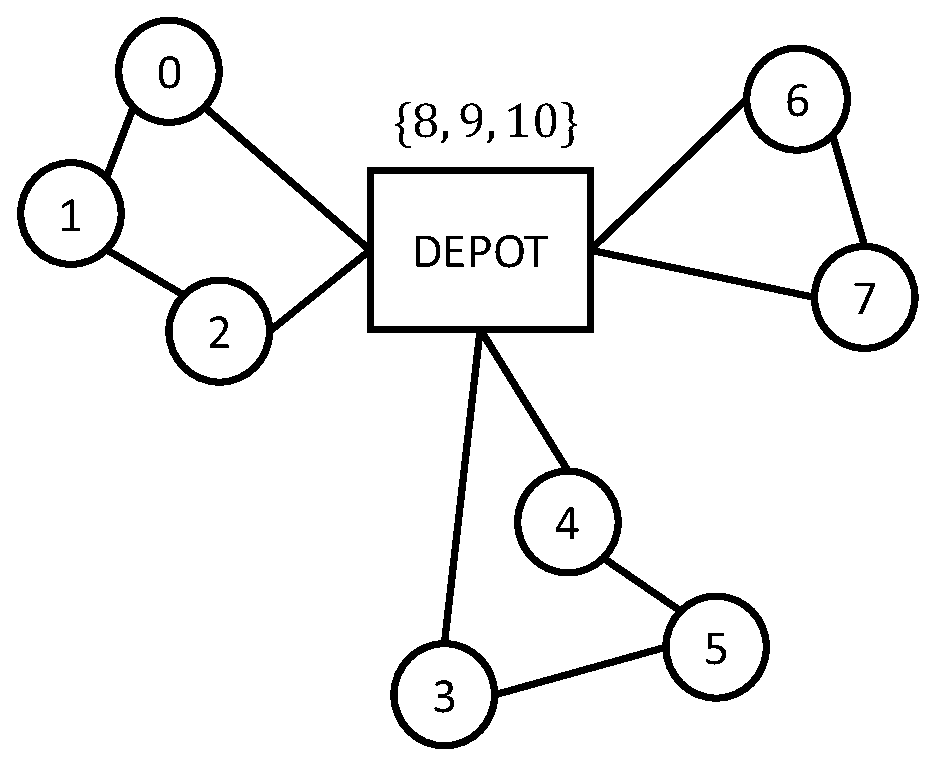
\includegraphics[width=0.5\textwidth]{cvrp_encoding.eps}
    \caption{Permutation Representation of CVRP, $N_c = 8$, $N_v = 4$}
	\label{fig:cvrp_encoding}
\end{figure}

Figure \ref{fig:cvrp_encoding} shows an example of this permutation representation. In this case, there are four vehicles ($N_v = 4$), and the number of customers is eight ($N_c =8$). Thus, the node numbers $0,1,2,...,7$ are for customers and numbers $8,9$ and $10$ are for the depot. The permutation $\pi = \{ 0,1,2,9,5,4,3,8,10,7,6 \}$ is interpreted as the three vehicle routes. In  this  sample, nodes $8$ and $10$ are adjacent and being virtual nodes, there is no distance between them and so no additional vehicle is assigned. Thus, three vehicles are used in this string. 

The objective function $F$, is defined as the sum of the distances traveled by each vehicle:
\begin{equation*}
	F(\pi_1, \pi_2, ... , \pi_n) = \sum_{i=1}^{N_v}{L_i} + K\cdot\sum_{i=1}^{N_v}{ \max{(0,L_i\frac{W_i-C}{C})}} \text{,}
\end{equation*}
where the first term of this equation is the total length of the routes of $N_v$ vehicle  and the second term is the penally for exceeding the weight capacity. This term is normalized by the capacity $C$ so that the penalty is applied consistently among variations in the absolute value. K is a constant value.

In  CVRP, the calculation of the objective function can be broken into calculation of the sum of each route distance of the vehicle. Then, the distance of each route is given by the relative ordering of the indices in the route. Dividing customers into different routes for vehicle increases difficulty of this problem than that in TSP. Since the objective function partially account on the relative ordering of the indices in the permutation, the information drawn from the relative ordering of each index is more significant. 

\subsection*{Vehicle Routing Problem With Time Window}
The vehicle routing problem with Time Window (VRPTW)\citep{toth2001vehicle} is the variation of CVRP. VRPTW has one more constraint than CVRP besides the capacity of the vehicle. The delivery locations have time windows within which the deliveries (or visits) must be made, or the routing scheme is failed. In the original VRPTW, the number of vehicle is also a variable of this optimization problem. Whereas, to only prove of the concept that MABMA can handle with more complicated problem, we reduce original VRPTW to a fixed vehicle VRPTW (fvVRPTW). That is, the optimal number of vehicle is given as CVRP does. 

The objective function of the fvVRPTW is like the one defined in Section \ref{section:cvrp} but the delay penalty is added:
\begin{equation*}
	F(\pi_1, \pi_2, ... , \pi_n) = \sum_{i=1}^{N_v}{L_i} + K\cdot\sum_{i=1}^{N_v}{ \max{\left(0,L_i\frac{W_i-C}{C} + D_i\right)}} \text{,}
\end{equation*}
where $D_i$ is the delay penalty of vehicle $i$. The delay penalty $D_i$ defined as the difference of the arrival time and the location closing time. For more specific definition, please refer to~\citep{toth2001vehicle}.

\subsection{Permutation Flow-Shop Scheduling Problem}
In the permutation flow-shop scheduling problem (PFSP)~\citep{gupta2006flowshop, french1982sequencing, allahverdi2008survey}, $n$ jobs $(i = 1,2,...,n)$ have to be scheduled on $m$ machines $(j = 1,2,...,m)$ in such a way that a given criterion is minimized. A job consists of $m$ operations and the $j$-th operation of each job must be processed on machine $j$ for a given specific processing time without interruption. The processing times are fixed, non-negative values and every job is available at time zero. At a given time, a job can start on the $j$-th machine when its $(j-1)$-th operation has finished on machine $(j-1)$, and machine $j$ is free. 

The goal of the optimization is to minimize the processing time of all the jobs, or in other words, to minimize the processing time of the last job. The solution is encoded as a permutation of length $n$ that represents the ordering in which the jobs are going to be processed. This means that for each machine the order of the jobs is the same and it is given as a permutation. For instance, in a problem of 4 jobs and 3 machines, the solution $(1,2,3,4)$ represents that job 1 is processed first, next job 2 and so on.

Let $p_{i,j}$ denote the processing time for job $i$ on machine $j$,and $c_{i,j}$ denote the
completion time of job $i$ on machine $j$. Then $c_{\pi_{i},j}$ is the completion time of the job scheduled in the $i$-th position in the sequence on machine $j$. $c_{\pi_{i},j}$ is computed as $c_{\pi_{i},j} = p_{\pi_i,j} + \max{ (c_{\pi_{i},j-1},c_{\pi_{i-1},j}) }$. Therefore, the objective function $F$ is defined as follows:
\begin{equation*}
	F(\pi_1, \pi_2, ... , \pi_n) = c_{\pi_n,m} \text{.}
\end{equation*}

As can be seen, the quality of a solution of the problem is given by the processing time of the last job $\pi_n$ in the permutation, since this job finishes the last. Even though the objective function is given by the time of this last job, the completion time of this last job depends on the ordering of the previous $\pi_1, \pi_2, ... , \pi_{n-1}$ jobs. Furthermore, in this problem, the value of the objective function can not be decomposed and depends on the position of each index in the permutation as well as on the whole order of the jobs.


\subsection{Linear Ordering Problem}
The linear ordering problem (LOP)~\citep{marti2011linear} arises in a large number of applications in a number of fields such as economy, sociology, graph theory, archaeology, and task scheduling~\citep{schiavinotto2004linear}. Two well known examples of LOP are the triangularization of input–output matrices of an economy, where the optimal ordering allows economists to extract some information about the stability of the economy, and the stratification problem in archaeology, where LOP is used to find the most probable chronological order

In LOP, for an given $n\times n$ matrix $C=[c_{ij}]$, and the goal is to determine a simultaneous permutation of the rows and columns of $C$ such that the sum of the superdiagonal entries is as large as possible (or equivalently, the sum of the subdiagonal entries is as small as possible). The solution of LOP is encoded as permutation of length $n$ where each index $\pi_i$ $(i=1,...,n)$ means that the values of the $\pi_i$-th row and column of the matrix are reallocated to the $i$-th position. The objective function is defined as follows:
\begin{equation*}
	F(\pi_1, \pi_2, ... , \pi_n) = \sum^{n}_{i=1}\sum^{n}_{j=i}{ c_{\pi_i\pi_j} } \text{.}
\end{equation*}
In this problem we can see that the contribution of an index $\pi_i$ to the objective function depends on the previous and posterior indices to it. However it does not depend on the order of these previous and posterior indices.


\subsection{Quadratic Assignment Problem}
The quadratic assignment problem (QAP) was introduced in~\citep{koopmans1957assignment} as a mathematical model for the location of a set of indivisible economical activities. Consider the problem of allocating a set of facilities to a set of locations, with the cost being a function of the distance and flow between the facilities, plus costs associated with a facility being placed at a certain location. The objective is to assign each facility to a location such that the total cost is minimized.

Specifically, for the two given $n\times n$ input matrices with real elements $H=[h_{ij}]$ and $D=[d_{kl}]$, where $h_{ij}$ is the flow between facilities $i$ and $j$, and $d_{kl}$ is the distance between locations $k$ and $l$. Given $n$ facilities, the solution of QAP is encoded as a permutation $\pi = (\pi_1, \pi_2,...,\pi_n)$ where each $\pi_i$ $(i =1,...,n)$ represents the facility that is allocated to the $i$-th location. The fitness of the permutation is given by the following objective function:
\begin{equation*}
	F(\pi_1, \pi_2, ... , \pi_n) = \sum^{n}_{i=1}\sum^{n}_{j=1}{ h_{ij}d_{\pi_i\pi_j} } \text{.}
\end{equation*}

In the solution of QAP, the absolute position of a facility (node) effects the cost between 
The quality of the solution is determined by the absolute position of each index (facility) in the permutation as regards the absolute position of the remaining indices.


